\chapter{Project management}

\minitoc

In order to successfully actualize this project, it is necessary to establish a common, high-level understanding of the team, external factors influencing the project, the project itself, and how to organize the work. The project management chapter is meant to document this.

\clearpage

\section{Team Structure}
We are a very small development team of just four team members. In a typical software development project, there are a large number of different roles, so each of us have to be assigned several different roles. We have defined a role for each responsibility that we believe to be important in our process. The person who is assigned a role should have an overview of the progress and have control over which tasks need to be done on their area. The work itself may be broken down into tasks so that these tasks can be executed by anyone from the team. The roles in our team are listed in the table \ref{table-teamroles}, overview of the roles is in table \ref{table-rolesoverview}.

\begin{table}
\centering
\begin{tabular}{ l  l }
  \hline
  \textbf{Team member} & \textbf{Roles} \\
  Ivo & Group leader, Customer and Advisor Contact, Scrum Master \\
  Oystein & Test Manager, QA Manager, Weekly Report Manager \\
  Oddvar & GUI Designer, Code Master, Meeting Secretary, Time Keeper \\
  Martin & System Architect, Report Manager \\
  \hline
\end{tabular}
\caption{Team role overview}
\label{table-rolesoverview}
\end{table}


\begin{table}
\caption{Team roles}
\begin{tabularx}{\textwidth}{ l X l }
  \textbf{Role} & \textbf{Description} & \textbf{Assignee} \\ 
  \hline \\ [-1.5ex]
  Team leader & Is responsible for administrative tasks and makes the final decisions. & Ivo \vspace*{0.7ex} \\ 
  \hline \\ [-1.5ex]
  Scrum Master & Shields the development team from external distractions and enforces the Scrum scheme.  & Ivo \vspace*{0.7ex}  \\ 
  \hline \\ [-1.5ex]
  Customer Contact & Handles communication with the customer. The customer should contact this person regarding general requests, questions and reminders. & Ivo (backup Martin) \vspace*{0.7ex}  \\ 
  \hline \\ [-1.5ex]
  Advisor Contact & Handles communication with the advisor. The advisor should contact this person regarding general requests, questions and reminders.  & Ivo (backup Martin) \vspace*{0.7ex} \\ 
  \hline \\ [-1.5ex]
  System Architect & Is responsible for the system architecture including distinctions and relations between subsystems and general code design choices. & Martin \vspace*{0.7ex} \\ 
  \hline \\ [-1.5ex]
  Code Master & Overall responsible for code management and structure. Managing branches in Git repository. & Oddvar \vspace*{0.7ex}  \\ 
  \hline \\ [-1.5ex]
  GUI Designer & Is responsible for the layout and design of graphical user interfaces. & Oddvar \vspace*{0.7ex} \\ 
  \hline \\ [-1.5ex]
  Test Manager & Is responsible for testing including unit tests, integration tests and usability tests. & Øystein \vspace*{0.7ex} \\ 
  \hline \\ [-1.5ex]
  Report Manager & Is responsible for delegating and overseeing work on the project report. & Martin \vspace*{0.7ex} \\ 
  \hline \\ [-1.5ex]
  Customer Representative & Participates in regular meetings to discuss the progress, project status and future tasks. Represents the customer. & Peder Kongelf \vspace*{0.7ex} \\ 
  \hline \\ [-1.5ex]
  Customer Technical Advisor & May be consulted about technical aspects of the project. & Stig Lau \vspace*{0.7ex} \\ 
  \hline \\ [-1.5ex]
  Advisor & Serves as a one-man steering committee for the project. & Meng Zhu \vspace*{0.7ex} \\ 
  \hline \\ [-1.5ex]
  Meeting Secretary & Is responsible for making sure notes get written and sent after each meeting with the advisor and customer. & Oddvar \vspace*{0.7ex} \\ 
  \hline \\ [-1.5ex]
  Quality Assurance Manager & Responsible for the process of agreeing on QA measures for the project and imposing these on the team  & Øystein \vspace*{0.7ex} \\ 
  \hline \\ [-1.5ex]
  Weekly Report Writer & Is responsible for finalizing the weekly report(s) for the advisor and customer, and getting these delivered for approval. Also responsible for meeting agendas and their delivery. & Øystein \vspace*{0.7ex} \\ 
  \hline \\ [-1.5ex]
  Time Keeper & Responsible for making sure that everybody is logging their work, and logging team activities. & Oddvar \vspace*{0.7ex} \\ 
  \hline
\end{tabularx}
\label{table-teamroles}
\end{table}

\section{Concrete Project Work Plan}
The course staff recommends us to work 25 person-hours per week and student. This project is estimated for 14 weeks. Since we at the moment have 4 group members in our group, the available effort will be $14*25*4=1400$ person hours including own reading, meetings, lectures, and seminars. The customer requested 5-7 students to handle this project, it is regrettably not likely that we will be supplied by one extra group member, so we must expect some more work hours divided on the four of us.

The first 4,5 weeks of the project were used on project planning, pre- study on the domain of the problem, to deduce user stories for the product backlog and to create the overall architecture of the system. The project is a proof of concept type of project, so it was important that we used a considerable amount of time on studying the domain of the problem and to find technologies that would solve the task as best as possible. Our Scrum process consists of 4 sprints, each 2 weeks long. In each sprint we had 200 work hours available, but a part of this will be used on report writing, project management, lectures and meetings. The two first sprint had an estimate of 130 hours available for development tasks, while the two last had an estimate of 140 work hours available. The last week will be used to evaluate the project, finish the report and to prepare the final presentation. The timeline of the project is outlined in Figure~\ref{figure:gantt}, and the WBS of the project is given in Table~\ref{table:wbs}.

\subsection{Activities}
\subsubsection{Lectures}
Lectures held by the course TDT4290 Customer Driven Project mainly aim to educate the students in the in the art of project management and the different tools used to handle this task in a better way. The lectures can give good insight into the workflow and how to avoid different issues, and should therefore be attended when the lecture involves tools used by the group or tools the group should consider using. After the lectures the group will reflect upon the presented material and if it is usable, or add value to our project, it will be integraded into the project.

\subsection {Milestones}
These are the deliverables and deadlines, that we have to take into account.
\begin {itemize}

\item August 21, Project start

\item October 14, Pre- Delivery: Deliver a copy of the Abstract, Introduction, the Pre-study and the Choice-of Lifecycle-model chapters to the external examiner (censor) and technical writing teacher. Also deliver the outline of the full report (Table of  Contents).

\item November 16, Code freeze: Final deadline for the completion of the implementation. The code should not be changed after this date.

\item November 22, Final Delivery: Project end. Deliver final report and present and demonstrate the final product at NTNU. Four printed and bound copies of  the project report should be delivered, as well as one electronic (PDF) copy.

\end {itemize}

\subsection {Sprints}
Sprint deadlines:
The pre- study, requirements, and testing plan activities should be finished before the start of the first sprint. If this is not the case the number sprints and their deadline might change. The start and end dates of each sprint is listed in Table~\ref{table:sprintdeadlines}

\begin{table}
\caption{Sprint Deadlines}
\centering
\begin{tabular}{ l l l }
\hline
Sprint Nr.		&Start		&End		\\
\hline
1		&24. September		&5. October		\\
2		&8. September			&19. October		\\
3		&22. October			&2. November		\\
4		&4. November			&18. November	\\
\hline
\end{tabular}
\label{table:sprintdeadlines}
\end{table}

\begin{figure}
\centering
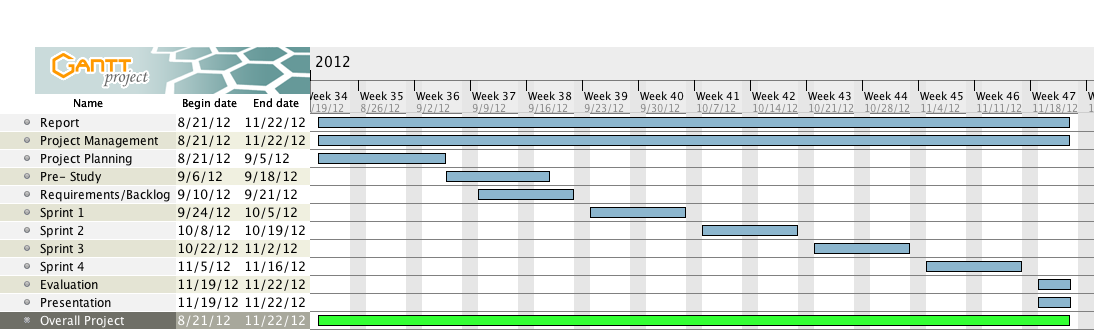
\includegraphics[width=6in]{image/gantt.png}
\caption{Gantt Chart}
\label{figure:gantt}
\end{figure}

\begin{table}
\caption{Work Breakdown Structure}
\centering
\begin{tabular}{ l l l l l }
\hline 
			&				&				&\multicolumn{2}{c}{Hours}		\\
 Task		& From date		&To date			&Est.			&Act.	                \\ 
\hline \\ [-2.0ex]
 The report     			&21/08/2012		&22/11/2012		&300		&320         	 \\
 Project Management	&21/08/2012		&22/11/2012		&180		&163		\\
 Project Planning		&21/08/2012		&05/09/2012		&100		&74		\\
 Lectures				&21/08/2012		&05/09/2012		&40			&50		\\	
 Pre- Study			&06/09/2012		&18/09/2012		&80			&89		\\
 Backlog				&10/09/2012		&21/09/2012		&60			&47		\\
 Architecture			&17/09/2012		&21/09/2012		&40			&51		\\
\hline \\ [-2.0ex]
 \bf{Sprint 1}			&\bf{24/09/2012}	&\bf{05/10/2012}	&\bf{130}		&\bf{128}	\\
 Planning				&				&				&20			&12		\\
 Design/Implementation	&				&				&90			&112	\\
 Testing				&				&				&20			&16		\\
\hline \\ [-2.0ex]
 \bf{Sprint 2}			&\bf{08/10/2012}	&\bf{19/10/2012}	&\bf{130}		&\bf{107.5}	\\
 Planning				&				&				&20			&22			\\
 Design/Implementation	&				&				&90			&65			\\
 Testing				&				&				&20			&20.5		\\
\hline \\ [-2.0ex]
 \bf{Sprint 3}			&\bf{22/10/2012}	&\bf{02/11/2012}	&\bf{140}		&\bf{95}		\\
 Planning				&				&				&20			&23		\\
 Design/Implementation	&				&				&100		&47		\\
 Testing				&				&				&20			&15		\\
\hline \\ [-2.0ex]
 \bf{Sprint 4}			&\bf{05/11/2012}	&\bf{16/11/2012}	&\bf{140}		&\bf{40}		\\
 Planning				&				&				&20			&14		\\
 Design/Implementation	&				&				&100		&19		\\
 Testing				&				&				&20			&7		\\
\hline \\ [-2.0ex]
 Evaluation			&19/11/2012		&22/11/2012		&30			&30		\\
 Final Presenation		&19/11/2012		&22/11/2012		&30			&30		\\
\hline \\ [-2.0ex]
 \bf{Total}			&				&				&\bf{1400}	&\bf{1224.5}		\\
\hline
\end{tabular}
\label{table:wbs}
\end{table}


\section{Constraints}
\subsection{Time}
The project must be completed within a timeframe of 13.6 weeks. Customer Driven Project is a 15 study points course, which makes it half a semester worth. The guideline is 24.3 work hours per person, per week. The project will be presented to a sensor on the 22th of November 2012.

\subsection{Knowledge about the problem}
Our problem is not well-explored and the customer cannot give us exact requirements. Thus, this is as much a research project as it is a software development project.

\subsection{Issues regarding  the system}
The customer has a huge workforce at their disposal, and it can be introduced to us through the customer. If there would appear a problem regarding the system we can’t handle ourselves, we can contact the customer and they can forward the issue to other sections of the corporation for analysis and problem solving. The communication regarding issues of this kind will usually be done per email. 

\subsection{Issues regarding the workflow}
The advisor can help us with issues regarding project management and workflow issues. If the group were to be stuck at some point, the advisor can jank the group out of the ditch and set it back on track. 

\section{Quality Assurance}
\subsection{Communication rules}
Communication with the customer is usually done by email. The customer will contact the assigned customer contact if anything else is not specified. The assigned customer contact is responsible for relaying any information received from the customer to the other group members as soon as possible. The customer contact is also responsible for sending any information from the group to the customer. Any communication from the customer demanding a reply, will be replied to within 8 hours. If any communication is sent from the group to the customer demanding a reply, this reply should be received by the group within 24 hours.

The same rules apply to the communication with the advisor.

\subsection{Internal Routines}
Each group member is responsible for logging all their work hours in the timekeeping system within 22:00 the same day. All group members are also responsible for checking the Skype group conversation within 22:00 Monday to Thursday, to see if any important information is posted there. If important information has to be delivered after this time, it will be sent by mail. All group members are required to check Redmine each day to check if any new task are assigned to that person.

\subsection{Deliverables}
All deliverables, including source code, documents and meeting notes, will be approved by at least two of the group members before it is sent for approval by either the advisor or the customer. All major phase documents must be approved by all the group members before it is relayed to the advisor for approval.

\subsection{Meetings}

\subsubsection{Advisor meetings}
Advisor meetings will occur every Thursday 09:15, unless anything else is specified, so the advisor gets updated on the latest work and progress of the project. The day before the meeting the group sends the advisor an agenda for the meeting and a status report of what is done since the last meeting. This will be sent to the advisor within 14:00 the day before the meeting. If this deadline is not sustained, any needed documents will be printed out and brought to the meeting. This lets the advisor enter the meeting prepared, and improve the efficiency of the meeting. Under the meeting issues regarding the work done, plans for next week and project management will be discussed. If there is a sprint-end-week the demo for this sprint will also be shown. Advisor notes will be written during the meetings, compiled and sent back to the advisor within 12:00 the following day.

\subsubsection{Customer meetings}
Customer meetings will occurs on demand, but usually weekly, and Thursdays 19:15 if there is a sprint-end-week, unless anything else is specified. Meetings will be scheduled at least 48 hours before the meeting starts, and confirmation from the customer should be received at least 24 hours before. An agenda for the meeting and a weekly progress report will be sent to the customer to keep him in the loop of the progress, and get prepared before the meetings. This documentation, including other documents needed for the meeting, will be sent by mail within 24 hours before the meeting. Since the customer is busy during work hours, the meetings are kept after 18:00 on weekdays, and after 12:00 in weekends. They will be kept over Skype, since the customer is located in Oslo. The meetings will be used to get the customer in the loop, clarify uncertainties and redirecting, if the direction of the project taken is not what the customer had in mind. The customer should also be included in the sprint planning meetings to help with use case prioritization. Customer notes will be written during the meetings, compiled and sent back to the customer within 12:00 the following day.

\subsubsection{Internal meetings}
Internal meetings will occur every Monday 12:15, unless anything else is specified. At this time all the group members are open for meetings. During these meetings the plans for the week will be discussed, workload divided and what was done last week. Notes will be taken and documented for later review. The group meet daily on skype to keep everyone up to date on the project progress and what will be done.

\subsubsection{Sprint planning meetings}
Sprint planning meetings will be held in the start of every sprint. Which use cases to handle and complete will be discussed here. The tasks will also be discussed with the customer so the customer can help prioritise the use cases and tell us which tasks they want us to complete first. The selected user stories along with their Work Breakdown Structure will be sent to the customer for approval.

\subsubsection{Sprint demonstration meetings}
Sprint demonstration meetings will be held Thursdays 19:15 in the end of the each sprint, unless anything else is specified. The group and the customer will be attending these meetings. An agenda will be sent to the customer, together with the weekly report and a link to the system, for the customer to test out. The demo will show the system and its new functionality. This lets the customer see the progress, and be able to come with inputs towards how their minds might differ from what has been produced, so the group can get on the right track if that is needed. This lets us make sure that we do not stray too far from the intended system. Since this is a meeting held with the customer the rules from the customer meetings will be held, so customer notes will be written during the meetings, compiled and sent back to the customer.

\subsection{Version Control}
GitHub was selected as the tool for version control in this project. All the relevant work that is produced will be pushed to the repository using git, including all the documents for the report, source code, images, diagrams, and so on. The group members will commit and push their changes on a regular basis, ensuring that the repository is always up to date and available.

\subsection{Document Templates}
The group has created templates for the following documents:

\begin{itemize}
\item Weekly status report \ref{statusreporttemplate}
\item Meeting agenda \ref{meetingagendatemplate}
\item Meeting notes \ref{meetingnotestemplate}
\end{itemize}

These templates are listed in the appendices.

\section{Scrum Process}
As explained in the pre- study, for this project we decided to use Scrum as our development methodology.  Scrum exists in many shapes and forms, following is a description of how we will carry out the process in this particular project.

\subsubsection{Roles}
The scrum process contains 3 distinct roles, the Scrum master, the product owner and the development team. The responsibilities of each role is explained in the pre- study. In this project the roles will be filled by
\begin{itemize}
\item Scrum master: Ivo
\item Product owner: Peder
\item Team: Rest of the group, including Ivo
\end{itemize}

\subsection{Key Elements}
Following is a description of the most important elements of the Scrum process
\newline
\newline
{\bf User stories} are a short simple descriptions of a desired feature. User stories are written by the different stakeholders of the project, with particular attention to the end user of the system. For the user stories we will follow a template developed by Mike Cohn, and its written in the form of: \begin{quote} "As a <type of user>, I want <some goal> so that <some reason>." \end{quote} The advantage of this form of user stories is that it provides a lot of information in one single sentence. It identifies who the end user is, what the end user wants, and the rationale behind it. 
\newline
\newline
The {\bf product backlog} consists of all the user stories currently derived for the product, and these user stories will be ordered according to their prioritisation from the customer. We will in cooperation with the customer derive the initial user stories for the product, that captures the desired functionality of the system. As the project goes on, new requirements or desired functionality almost certainly will be discovered. New user stories should be created and added to the product backlog. Also the prioritisation of the user stories might change form the customer point of view, and this should be updated in the backlog as a result. The {\bf sprint backlog} contains all the user stories that were picked during the planning meeting. Any user stories remaining at the end of the sprint will carry over in the next one, or put back in the product backlog.

\subsection{Process}

\subsubsection{Scrum Planning Meeting}
Each sprint will last for two weeks and will start with a sprint planning meeting. In this meeting the work to be done in the following sprint will be discussed and decided on. The customer should be heavily involved in this process, picking user stories from the top of the product backlog, as these have the highest priorities. Each user story should contain an estimate on their workload, and the number of user stories picked depends on these numbers. The scrum planning meeting is in essence a preparation of the sprint backlog.

\subsubsection{Daily Meetings}
During the sprint daily scrum meetings will be carried out. Ideally should be held the at the same time every day, but in our case this will be difficult as we all have different schedules. We will however set a time for each day that suits all, and these times will be consistent. In the daily meetings the team members will present 3 things to each other:
\begin{itemize}
\item What have you done since yesterday?
\item What are you planning to do today?
\item What issues are you currently facing?
\end{itemize}

\subsubsection{Sprint Demo}
At the end of the sprint, a demonstration to the product owner will be held. In this demo we will present what we, the team, has completed during the sprint. We should present something that works, meaning only complete work should be shown to the product owner. The product owner will provide feedback on the finished solutions, and let us know if any changes needs to be made.

\subsubsection{Sprint review}
The sprint review will be performed by the team following a sprint. In these evaluations we will ask ourselves two main questions, what went well this sprint, and what can be improved in the next sprint.


\section{Risks}
We have tried to identify potential risks early, and document these, by specifying
\begin{itemize}
\item The activity during which they may occur and disrupt the workflow
\item The risk factor itself; the unfortunate circumstance that might arise
\item Impact of the risk, ranked from low(minor inconvenience) to significant(will cause disruption, but we can recover) to critical(must be resolved to prevent project failure)
\item Description of the consequences of the risk
\item Probability ranked from very low(extremely unlikely) to very high(to be expected).
\item Countermeasures to both prevent and recover from the problems
\item Any deadline for when the problem must be resolved
\item The person responsible for taking action on the risk
\end{itemize}
Full tables describing our identified risks are listed in the appendices.


\section{Tool Selection}
After detailed study of some tools, we decided to use tools and frameworks listed in table \ref{table-tools}. In communication and collaboration tools section, the main reason for choosing these tools were last experiences with these - most of us already used these tools in work or in other projects, so we do not have to learn to use something new. 

LaTeX software was used to write this report, although most of the team members did not use LaTeX before We decided to use it, because it has a lot of advantages. It is easy to colaborate on source code and use git to track the changes, the result pdf document looks better, than the one produced in other tools, there is automatic referencing of tables, figures and citations. Also the table of contents, tables and figures is automatically generated. Also, using LaTeX was recommended by the customer.

For backend of the system, we wil be using MongoDB in combination with Node.js. Both are extremely effective, scalable and easy to learn. Also they share the same runtime, so the deployment process on the server is simplified. MongoDB and Node.js are newand up-to-date technologies, that are getting more and more used in web applications. NoSQL schemeless MongoDB allows to store any data frontend requires and also the data migration is easy. Node.js can communicate with MongoDB using JavaScrip libraries and offer the data through standard REST interface. Client can retrieve the data from server via HTTP protocol using Ajax with JavaScript and present it to the user. The user interface is written using HTML, CSS and JavaScript.

\begin{table}
\centering
\begin{tabular}{ l l}
\textbf{Part of project}  & \textbf{Technology} \\
\hline
Communication & Skype, Google Groups, Google Calendar \\
Document colaboration & Google Docs, Google Drive \\
Code colaboration & Git + Github \\
Time tracking and mamangement & Redmine \\
Report & Latex \\
Backend & Node.js \\
Database & MongoDB \\
Communication & PubNub \\
Client & JavasScript + JQuery, HTML, CSS \\
\hline
\end{tabular}
\caption{Tools used in project}
\label{table-tools}
\end{table}
